% =====================================================================
% Draft for IEEE Open Journal of the Computer Society (OJ-CS).
% Written with IEEEtran (journal mode) so it compiles anywhere. Before
% submission, move the content into the IEEE Open Journals template from
% the IEEE Author Center (limit: 12 pages for regular papers).
% All numbers in tables come from paper/make_tables.py.
% Items marked [TODO] must be completed by the authors.
% =====================================================================
\documentclass[journal]{IEEEtran}
\usepackage{amsmath,amssymb}
\usepackage{booktabs}
\usepackage{graphicx}
\usepackage{cite}
\usepackage{url}
\usepackage{iftex}
\ifXeTeX
  \usepackage{fontspec}
  \setmainfont{texgyretermes}[Extension=.otf, UprightFont=*-regular, BoldFont=*-bold,
    ItalicFont=*-italic, BoldItalicFont=*-bolditalic]
\fi
\usepackage{xcolor}
\usepackage[hidelinks]{hyperref}
% uppercase colour name: IEEEtran upper-cases running heads, which would turn "red" into "RED"
\definecolor{TODOC}{rgb}{0.8,0,0}
\newcommand{\todo}[1]{\textcolor{TODOC}{[TODO: #1]}}
\newtheorem{proposition}{Proposition}
\newtheorem{definition}{Definition}
\DeclareMathOperator*{\argmax}{arg\,max}

\begin{document}

\title{Revisiting SINdex: Label Validity, a Corrected\\ Inconsistency Measure, and Contradiction-Aware\\ Clustering for Black-Box Hallucination Detection}

\author{Sulaxan Jadhav \todo{add co-authors, if any, in order}%
\thanks{The authors are with the Symbiosis School of Economics, Symbiosis International (Deemed University), Pune, India. \todo{If any co-author has a different affiliation, list it separately.}}%
\thanks{Corresponding author: Sulaxan Jadhav, Assistant Professor (e-mail: sulaxan.jadhav@sse.ac.in; ORCID: 0000-0003-2500-6030).}}

\markboth{IEEE Open Journal of the Computer Society, \todo{year}}{Jadhav: Revisiting SINdex}

\maketitle

\begin{abstract}
Sampling-based black-box detectors flag a large language model (LLM) answer as a likely hallucination when repeated samples disagree in meaning. SINdex, a recent detector of this kind, clusters sentence embeddings of sampled answers and scores them with a cohesion-weighted entropy, and reports gains of up to 9.3\% AUROC over semantic entropy. We revisit SINdex and make four contributions. (i)~We show that its theoretical justification does not hold: the cohesion-weighted proportions are not a probability vector, the score \emph{decreases} as clusters loosen whenever a cluster holds less than $1/e$ of the samples, and singleton clusters are undefined. We propose SINdex++, an additive form that is provably monotone in cohesion and lower-bounded by the cluster entropy. (ii)~We show that the evaluation protocol's correctness labels, based on an embedding-cosine threshold, are unreliable: against a 201-item reference annotation (a human re-annotation of a random subset agreed on 40/40 items), they reach 56.8\% accuracy (Cohen's $\kappa=0.26$), whereas a majority vote of three LLM judges reaches 97.3\% ($\kappa=0.94$). (iii)~Re-evaluating on 2 open models $\times$ 3 question-answering datasets with validated labels, SINdex's lead over plain cluster entropy falls from $+0.040$ to a non-significant $+0.007$ AUROC, and SINdex is statistically tied with the earlier EigV baseline. (iv)~We propose a contradiction-aware clustering step that runs a small natural-language-inference model only on borderline answer pairs; it improves AUROC by $+0.014$ on average (95\% CI $[+0.005, +0.025]$, $p<0.001$), with gains in 5 of 6 settings. Code, generations and labels are released.
\end{abstract}

\begin{IEEEkeywords}
Hallucination detection, large language models, semantic uncertainty, uncertainty quantification, evaluation methodology, natural language inference.
\end{IEEEkeywords}

% =====================================================================
\section{Introduction}
\IEEEPARstart{L}{arge} language models (LLMs) produce fluent text that is sometimes factually wrong, a failure commonly called \emph{hallucination}~\cite{ji2023survey,huang2025survey}. When only the generated text is available, as with commercial APIs, a practical signal is self-consistency: if an LLM answers the same question several times and the answers disagree in meaning, the model is probably uncertain and the answer is more likely to be wrong~\cite{manakul2023selfcheckgpt,kuhn2023semantic,farquhar2024detecting}. Semantic entropy~\cite{kuhn2023semantic,farquhar2024detecting} groups sampled answers by bidirectional entailment and computes the entropy over meaning clusters. SINdex~\cite{abdaljalil2026sindex} replaces entailment-based grouping with hierarchical clustering of sentence embeddings, weights each cluster's share by its internal cosine cohesion, and reports AUROC gains of up to 9.3\% over semantic entropy with a 60-fold speed-up of the grouping step.

This paper revisits SINdex from three angles: its theory, its evaluation protocol, and its main design choice. We find that (a)~its stated theoretical property is false in the regime where hallucinations occur, (b)~the labels used to decide which answers are hallucinations are wrong on a large fraction of correct but verbose answers, and that this labelling, rather than the cohesion weighting, accounts for most of SINdex's reported advantage, and (c)~replacing embedding similarity entirely is unnecessary: a small entailment model applied only to borderline pairs recovers the cases embeddings miss (different numbers, dates or negations that look similar in embedding space).

\textbf{Contributions.}
\begin{itemize}
\item[\textbf{C1}] A counterexample and a closed-form characterisation showing that SINdex is not monotone in cluster cohesion, and \textbf{SINdex++}, an additive inconsistency measure with proven monotonicity and bounds (Section~\ref{sec:theory}).
\item[\textbf{C2}] A \textbf{contradiction-aware clustering} step that vetoes merges between borderline-similar answers flagged as contradictory by a small NLI cross-encoder (Section~\ref{sec:method}).
\item[\textbf{C3}] A \textbf{label-validity audit}: a 201-item reference annotation, partially re-annotated by a human, comparing seven labelling rules, and a three-judge majority vote with a revised judge prompt (Section~\ref{sec:labels}).
\item[\textbf{C4}] A \textbf{re-evaluation} on Qwen2.5-7B and Llama-3.1-8B over TriviaQA, Natural Questions and SQuAD with paired, pooled bootstrap tests, including two negative results (adaptive cluster cut, early stopping) (Section~\ref{sec:results}).
\end{itemize}

% =====================================================================
\section{Related Work}
\textbf{Hallucination detection.} Surveys~\cite{ji2023survey,huang2025survey} distinguish white-box detectors that read hidden states~\cite{chen2024inside}, gray-box detectors that use token probabilities~\cite{kadavath2022language}, and black-box detectors that use only sampled text~\cite{manakul2023selfcheckgpt,lin2024generating}. Black-box detectors apply to any API-served model.

\textbf{Semantic uncertainty.} Semantic entropy~\cite{kuhn2023semantic,farquhar2024detecting} clusters answers by bidirectional entailment and computes entropy over clusters. Kernel language entropy~\cite{nikitin2024kernel} replaces hard clusters by a semantic kernel. Lin et al.~\cite{lin2024generating} build a similarity graph over samples and propose Degree, Eccentricity and EigV scores; these are strong black-box baselines that SINdex does not compare against. SINdex~\cite{abdaljalil2026sindex} clusters sentence embeddings~\cite{reimers2019sbert} with average-linkage agglomerative clustering and weights cluster shares by intra-cluster cosine similarity.

\textbf{Evaluating detectors.} Detectors are scored by AUROC against correctness labels of the most-likely answer. Labels are usually produced automatically: string match, embedding similarity, or an LLM judge~\cite{farquhar2024detecting,zheng2023judging}. Because every reported number depends on these labels, we audit them directly.

% =====================================================================
\section{SINdex in Brief}\label{sec:background}
Given a question $q$, the LLM is sampled $P$ times at temperature~1, yielding answers $g_1,\dots,g_P$. Each string $s_i = q\,[\mathrm{SEP}]\,g_i$ is embedded with a sentence encoder; answers are clustered by average-linkage agglomerative clustering on cosine distance $1-\cos(\cdot,\cdot)$ with a fixed cut at distance $0.05$, giving clusters $C_1,\dots,C_k$ with shares $p_i = |C_i|/P$. With $\bar c_i$ the mean pairwise cosine similarity inside $C_i$, SINdex is
\begin{equation}
\mathrm{SINdex} = -\sum_{i=1}^{k} p_i' \log p_i', \qquad p_i' = p_i\,\bar c_i. \label{eq:sindex}
\end{equation}
The original paper argues that $p'\le p$ element-wise implies that $p'$ is majorized by $p$, so by Schur-concavity of entropy $\mathrm{SINdex}\ge H(p)$, and that the score decreases monotonically as cohesion increases~\cite{abdaljalil2026sindex}.

The most-likely answer (sampled at temperature $0.1$) is labelled a hallucination unless its embedding has cosine similarity $>0.95$ with the reference answer, using the same encoder as the detector~\cite{abdaljalil2026sindex}.

% =====================================================================
\section{Theory: SINdex is Not Monotone; SINdex++}\label{sec:theory}
\begin{proposition}\label{prop:flaw}
For a cluster with share $p_i>0$ and cohesion $\bar c_i\in(0,1]$,
\begin{equation}
\frac{\partial\,\mathrm{SINdex}}{\partial \bar c_i} = -p_i\bigl(1+\log(p_i\bar c_i)\bigr),
\end{equation}
which is \emph{positive} whenever $p_i\bar c_i<1/e$. Hence SINdex increases with cohesion for every cluster holding less than $1/e\approx 37\%$ of the samples, and $\mathrm{SINdex}<H(p)$ is possible.
\end{proposition}
\begin{IEEEproof}
Differentiate $-x\log x$ at $x=p_i\bar c_i$ and apply the chain rule. For the second claim, take $p=(0.2,\dots,0.2)$ with $k=5$ and $\bar c_i=0.8$: $\mathrm{SINdex}=1.466$ while $H(p)=\log 5=1.609$.
\end{IEEEproof}

The majorization argument fails because $p'$ does not sum to one; majorization is defined between vectors with equal sums~\cite{marshall2011inequalities}. Table~\ref{tab:cex} shows the effect: with five clusters of two answers, looser clusters \emph{lower} the score, the opposite of the stated property, while with two clusters of five the stated direction holds. Fig.~\ref{fig:theory} plots both measures over a range of cohesion values. Many clusters with few members is precisely the uncertain regime that matters for hallucination detection. In addition, $\bar c_i$ is $0/0$ for singleton clusters, which are common (Section~\ref{sec:results}); the original paper does not specify a convention.

\begin{table}[t]\centering
\caption{SINdex for $P=10$ answers as cluster cohesion decreases. With small clusters ($p_i<1/e$) the score falls when clusters become looser.}
\label{tab:cex}\small
\begin{tabular}{lccc}\toprule
Clusters & $\bar c=1.0$ & $\bar c=0.9$ & $\bar c=0.8$\\\midrule
$2\times 5$ answers ($p_i=0.5$) & 0.693 & 0.719 & 0.733\\
$5\times 2$ answers ($p_i=0.2$) & 1.609 & 1.543 & 1.466\\
\bottomrule\end{tabular}
\end{table}

\begin{figure}[t]\centering
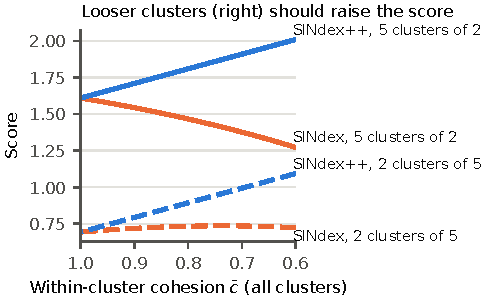
\includegraphics[width=\columnwidth]{figures/theory.pdf}
\caption{SINdex (orange) and SINdex++ (blue) as all clusters become looser (left to right). With five small clusters (solid), SINdex \emph{falls} as cohesion drops, contradicting the property claimed in~\cite{abdaljalil2026sindex}; SINdex++ rises in both configurations (Proposition~\ref{prop:pp}).}
\label{fig:theory}
\end{figure}

\begin{definition}[SINdex++]
With singleton cohesion defined as $\bar c_i=1$ (zero internal dispersion) and $\lambda>0$,
\begin{equation}
\mathrm{SINdex}^{++} = H(p) + \lambda\sum_{i=1}^{k} p_i\,(1-\bar c_i). \label{eq:sindexpp}
\end{equation}
\end{definition}
The second term is the expected within-cluster dispersion of a randomly drawn sample.

\begin{proposition}\label{prop:pp}
For $\bar c_i\in[0,1]$ and $\lambda>0$: (a)~$H(p)\le \mathrm{SINdex}^{++}\le \log k+\lambda$; (b)~equality on the left holds iff every non-empty cluster has $\bar c_i=1$; (c)~$\partial\,\mathrm{SINdex}^{++}/\partial \bar c_i = -\lambda p_i<0$, so the score strictly decreases as any cluster becomes more cohesive.
\end{proposition}
\begin{IEEEproof}
Each term $p_i(1-\bar c_i)\in[0,p_i]$, so the penalty lies in $[0,\lambda]$ and is zero iff all $\bar c_i=1$; $H(p)\le\log k$. Part (c) is immediate from linearity.
\end{IEEEproof}
We use $\lambda=1$ throughout and do not tune it. Section~\ref{sec:results} shows that the correction, although it changes the score on most questions, has no measurable effect on AUROC at the paper's clustering threshold, because cohesion inside clusters cut at cosine $0.95$ is close to~1.

% =====================================================================
\section{Contradiction-Aware Clustering}\label{sec:method}
Embedding similarity is weak at telling apart answers that differ in a number, date or negation: ``born in 1879'' and ``born in 1897'' are close in embedding space but contradict each other. Entailment models handle such cases but are expensive when applied to all $P(P-1)/2$ pairs~\cite{kuhn2023semantic}. We combine the two (Fig.~\ref{fig:pipeline}).

\begin{figure*}[t]\centering
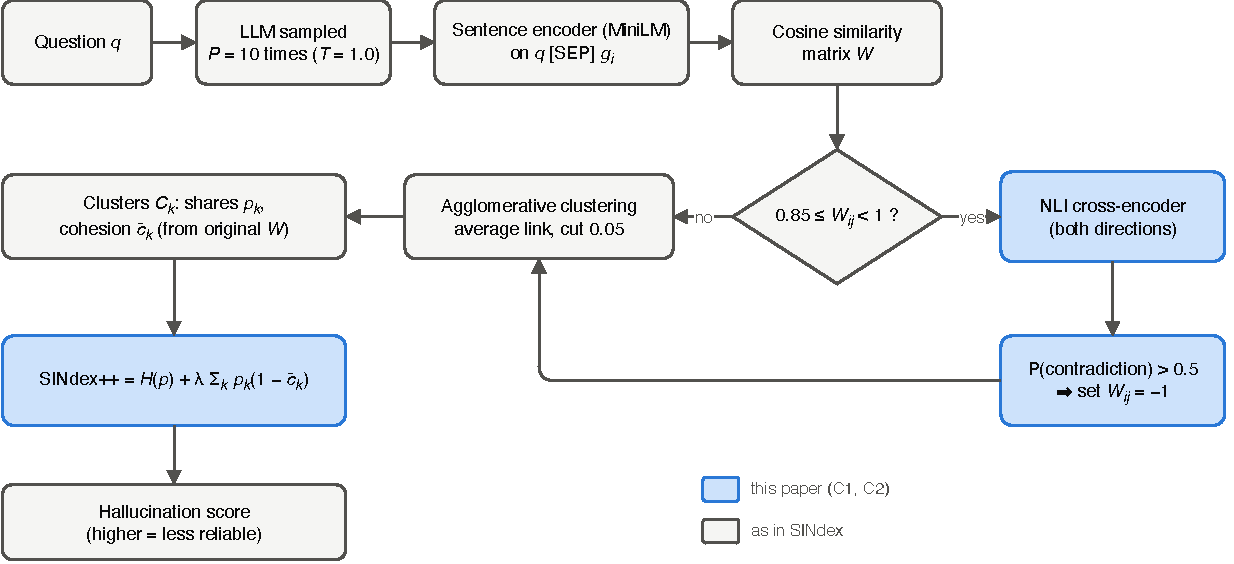
\includegraphics[width=0.95\textwidth]{figures/pipeline.pdf}
\caption{Contradiction-aware SINdex++. Grey steps are as in SINdex~\cite{abdaljalil2026sindex}; blue steps are ours. Only answer pairs that are already similar in embedding space are passed to the NLI model; pairs it judges contradictory cannot be merged. Cohesion is computed on the original similarities. Drawn in draw.io.}
\label{fig:pipeline}
\end{figure*}

\textbf{NLI veto.} We compute the cosine similarity matrix $W$ as in SINdex. For each pair $(i,j)$ with $W_{ij}\in[\tau_{\mathrm{lo}},1]$ and non-identical text, we query a cross-encoder NLI model in both directions. If the contradiction probability exceeds $0.5$ in either direction, we set $W_{ij}=-1$ (distance 2) before linkage, so that the two answers cannot be merged at the clustering threshold. Cohesion $\bar c_i$ is still computed on the original $W$. We use $\tau_{\mathrm{lo}}=0.85$ and the 140M-parameter cross-encoder \texttt{nli-deberta-v3-small}~\cite{he2023debertav3}; these values were fixed in advance and not tuned on test data.

\textbf{Worked example.} Fig.~\ref{fig:example} shows a TriviaQA question on which Qwen2.5-7B answers ``30'' five times, ``33'' three times and ``11'' (correct) twice. All ten answers have pairwise cosine similarity $\ge 0.944$, so embedding-only clustering forms a single cluster and SINdex is $0.016$: the detector reports high confidence in a wrong answer. The NLI model flags the differing numbers as contradictions, the answers split into three clusters, and the score rises to $1.039$ (from the 37th to the 64th percentile of scores on this dataset).

\begin{figure*}[t]\centering
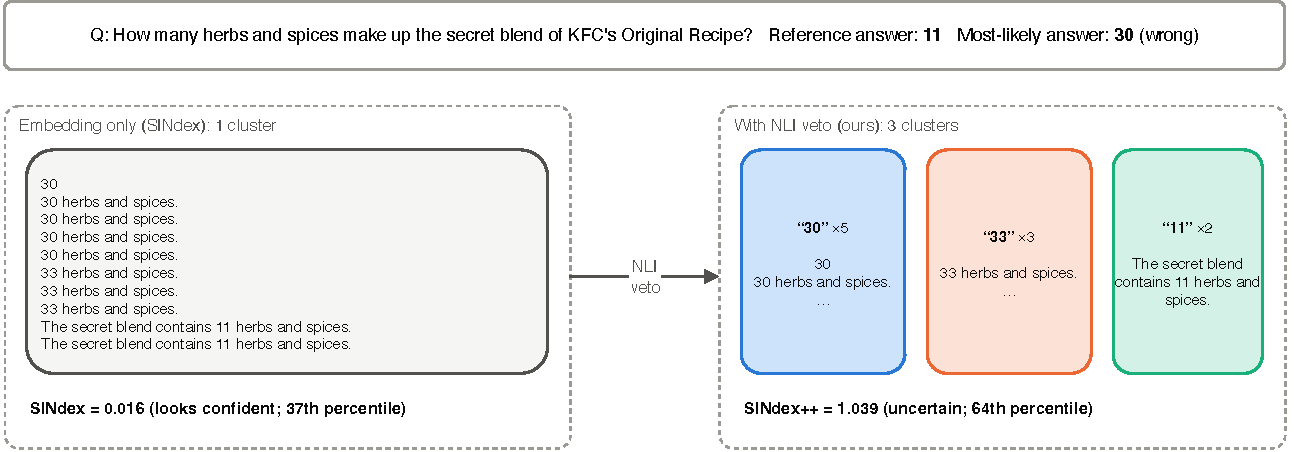
\includegraphics[width=0.85\textwidth]{figures/example.pdf}
\caption{A real example (Qwen2.5-7B, TriviaQA). Embedding similarity merges answers that state different numbers; the NLI veto separates them and the score correctly signals uncertainty. Drawn in draw.io.}
\label{fig:example}
\end{figure*}

\textbf{Cost.} Recomputed offline on the Qwen2.5-7B generations, the similarity band $[0.85,1]$ contains 45\%, 58\% and 39\% of all answer pairs on TriviaQA, NQ and SQuAD, and the veto changes the clustering of 19\%, 26\% and 5\% of questions. Checking a band pair needs two NLI calls, so the step uses 35--52 calls per question instead of 90 for all pairs in both directions. On an Apple~M1 GPU this takes 0.53--0.74\,s per question, against 0.02--0.04\,s for the embeddings. A narrower band would cut the cost further; we did not tune it.

\textbf{Other variants (negative results).} \emph{Adaptive cut}: instead of the fixed distance $0.05$, cut the dendrogram in the middle of the largest gap between merge heights in $[0.02,0.30]$. \emph{Early stopping}: score the first three samples, stop if they form one cluster or if the score changes by less than $0.05$ for two consecutive added samples, otherwise continue up to $P$. Both are evaluated offline on the cached samples.

\textbf{Baselines.} Cluster entropy $H(p)$ using the same clusters (a discrete semantic-entropy analogue with embedding clusters); Degree, Eccentricity and EigV of Lin et al.~\cite{lin2024generating} on the cosine graph clipped to $[0,1]$ (Eccentricity uses eigenvectors with eigenvalue below $0.9$); and, as a gray-box reference, length-normalised predictive entropy from the samples' log-likelihoods.

% =====================================================================
\section{Label Validity}\label{sec:labels}
\textbf{Labelling rules.} We compare: the SINdex rule (embedding cosine $>0.95$ to any reference answer, same encoder as the detector); exact match after SQuAD normalisation; token F1 $\ge 0.5$; exact match or normalised containment of a reference answer (``EM$\lor$contains''); and three LLM judges.

\textbf{LLM judges.} We use Qwen2.5-7B-Instruct, Qwen2.5-14B-Instruct (AWQ) and Granite-3.1-8B-Instruct, the last from a different model family than either generator. A first judge prompt in the style of~\cite{farquhar2024detecting} wrongly rejected correct answers phrased as full sentences or with extra words (e.g., ``Westwood One carried the game throughout North America'' for the reference ``Westwood One''). The revised prompt states that an answer is correct if it gives the reference answer or an equivalent, including inside a longer sentence, and wrong if it names a different entity, number or date, contradicts the reference, or does not answer. Judges decode greedily; we parse the first standalone yes/no. The label used for evaluation is the majority vote of the three judges.

Fig.~\ref{fig:evaluation} summarises the labelling and validation workflow.

\begin{figure*}[t]\centering
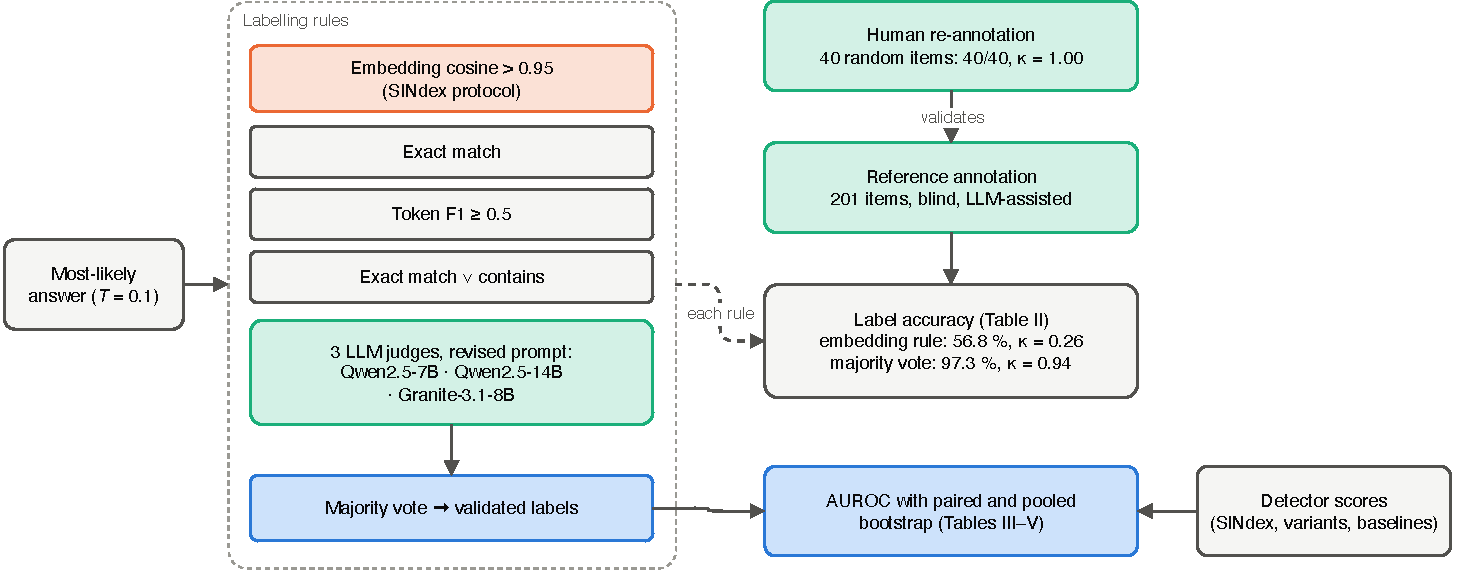
\includegraphics[width=0.78\textwidth]{figures/evaluation.pdf}
\caption{Labelling and validation workflow. Every labelling rule is scored against a reference annotation that a human re-annotation confirms; detectors are then evaluated with the validated (majority-vote) labels. Orange: the original protocol. Drawn in draw.io.}
\label{fig:evaluation}
\end{figure*}

\textbf{Reference annotation.} We drew 201 Qwen2.5-7B answers: 50 random questions per dataset plus 17 per dataset on which the judge majority and EM$\lor$contains disagree (a deliberately hard subset). Items were shuffled and shown without any model label. The reference labels were produced with the assistance of an LLM (Claude, Anthropic) following a written rubric; 14 items whose reference answer was itself wrong or ambiguous were marked unsure and excluded. To validate the reference, a human annotator independently labelled a random subset of 40 decided items. Agreement was 40/40 (Cohen's $\kappa=1.00$~\cite{cohen1960kappa}; 95\% Clopper--Pearson lower bound on agreement 0.91~\cite{clopper1934use}). \todo{Add a second human annotator on the same 40 items if possible, and report inter-annotator agreement.}

\begin{table}[t]\centering
\caption{Accuracy of labelling rules against the reference annotation (random subset, $n=146$; Qwen2.5-7B answers on all three datasets). $\kappa$: Cohen's kappa.}
\label{tab:labels}\small\setlength{\tabcolsep}{4pt}
\begin{tabular}{lcc}\toprule
Labelling rule & Accuracy & $\kappa$\\\midrule
Embedding cosine $>0.95$ (SINdex~\cite{abdaljalil2026sindex}) & 0.568 & 0.26\\
Exact match & 0.589 & 0.29\\
Token F1 $\ge 0.5$ & 0.719 & 0.47\\
Exact match $\lor$ contains & 0.945 & 0.88\\
Judge: Qwen2.5-7B & 0.966 & 0.93\\
Judge: Qwen2.5-14B & 0.925 & 0.84\\
Judge: Granite-3.1-8B & 0.986 & 0.97\\
Majority of 3 judges (ours) & 0.973 & 0.94\\
\bottomrule\end{tabular}\end{table}

Table~\ref{tab:labels} reports accuracy on the 146 decided random items. The SINdex labelling rule reaches 56.8\% accuracy ($\kappa=0.26$): of the 94 answers in this subset that are correct, it marks 63 (67\%) as hallucinations, because a correct sentence-length answer rarely reaches cosine $0.95$ with a short reference answer. Exact match fails for the same reason. The three judges reach 92.5--98.6\%, and their majority 97.3\% ($\kappa=0.94$). On the hard subset the majority is less reliable (it over-calls hallucinations), so we also report results with a stricter \emph{consensus} label (judges' majority \emph{and} EM$\lor$contains both say wrong).

% =====================================================================
\section{Experimental Setup}\label{sec:setup}
\textbf{Models and data.} Generators: Qwen2.5-7B-Instruct~\cite{qwen2025} and Llama-3.1-8B-Instruct~\cite{dubey2024llama} (weights from an ungated redistribution of the official checkpoint, used under the Llama~3.1 Community License). Datasets: TriviaQA (\texttt{rc.nocontext}, validation)~\cite{joshi2017triviaqa}, Natural Questions open~\cite{kwiatkowski2019natural,lee2019latent} and SQuAD~v1.1 with context~\cite{rajpurkar2016squad}. As in~\cite{abdaljalil2026sindex}, we sample 400 questions per dataset (seed 0); TriviaQA contains duplicate question identifiers, leaving 388 unique questions.

\textbf{Generation.} Prompt: ``Answer the following question as briefly as possible.'' followed by the context (SQuAD only), the question, and ``Answer:'', wrapped in each model's chat template. Most-likely answer at temperature $0.1$; $P=10$ samples at temperature $1.0$, top-$p=1$; at most 64 new tokens. Inference uses vLLM~\cite{kwon2023efficient} on one NVIDIA L4 (24\,GB).

\textbf{Detector settings.} Encoder \texttt{all-MiniLM-L6-v2}~\cite{reimers2019sbert} on $q\,[\mathrm{SEP}]\,g$; average linkage; distance cut $0.05$; $\lambda=1$. All settings follow~\cite{abdaljalil2026sindex} or were fixed before evaluation; no hyperparameter was tuned on the evaluation questions.

\textbf{Statistics.} AUROC with 95\% percentile bootstrap intervals (2{,}000 resamples)~\cite{efron1994introduction}. Differences between detectors use a paired bootstrap on the same resampled questions, one-sided $p$ for $\Delta\le 0$. For pooled results we resample questions within each of the six model--dataset runs and average the per-run differences (4{,}000 resamples).

% =====================================================================
\section{Results}\label{sec:results}
\begin{table*}[t]\centering
\caption{AUROC for hallucination detection with validated labels (majority of three LLM judges). 400 questions per dataset (TriviaQA: 388 unique), $P{=}10$ samples. Bold: best black-box score per column. $^{\dagger}$: better than SINdex, one-sided paired bootstrap $p<0.05$ (2{,}000 resamples).}
\label{tab:main}\small
\begin{tabular}{lcccccc}\toprule
 & \multicolumn{3}{c}{Qwen2.5-7B} & \multicolumn{3}{c}{Llama-3.1-8B}\\
\cmidrule(lr){2-4}\cmidrule(lr){5-7}
Method & TriviaQA & NQ & SQuAD & TriviaQA & NQ & SQuAD\\\midrule
SINdex~\cite{abdaljalil2026sindex} & 0.808 & 0.779 & 0.649 & 0.858 & 0.705 & 0.799\\
SINdex++ (ours, C1) & 0.808 & 0.779 & 0.649 & 0.858 & 0.705 & 0.799\\
SINdex++ + NLI veto (ours, C2) & \textbf{0.826}$^{\dagger}$ & \textbf{0.797}$^{\dagger}$ & 0.640 & \textbf{0.868}$^{\dagger}$ & \textbf{0.716} & \textbf{0.836}\\
SINdex++ + adaptive cut & 0.792 & 0.755 & 0.648 & 0.824 & 0.664 & 0.797\\
SINdex++ + early stop & 0.781 & 0.785 & 0.576 & 0.839 & 0.703 & 0.797\\
\midrule
Cluster entropy & 0.798 & 0.779 & \textbf{0.655} & 0.851 & 0.706 & 0.770\\
EigV~\cite{lin2024generating} & 0.805 & 0.778 & 0.652 & 0.847 & 0.691 & 0.789\\
Degree~\cite{lin2024generating} & 0.805 & 0.779 & 0.652 & 0.848 & 0.693 & 0.789\\
Eccentricity~\cite{lin2024generating} & 0.734 & 0.687 & 0.630 & 0.738 & 0.607 & 0.762\\
Predictive entropy (gray-box) & 0.779 & 0.749 & 0.616 & 0.846 & 0.712 & 0.796\\
\bottomrule\end{tabular}\end{table*}
\begin{table}[t]\centering
\caption{Pooled comparison over 2 models $\times$ 3 datasets: mean $\Delta$AUROC with 95\% CI from a stratified paired bootstrap (4{,}000 resamples per run) and two-sided $p$-value. Validated labels unless stated.}
\label{tab:pooled}\scriptsize\setlength{\tabcolsep}{2.5pt}
\begin{tabular}{lcc}\toprule
Comparison & $\Delta$AUROC [95\% CI] & $p$\\\midrule
NLI veto (C2) $-$ SINdex & $+0.014$ [$+0.005$, $+0.025$] & 0.001\\
SINdex++ (C1) $-$ SINdex & $+0.000$ [$-0.001$, $+0.001$] & 0.949\\
SINdex $-$ clust.\ ent.\ (paper labels) & $+0.040$ [$+0.030$, $+0.050$] & $<$0.001\\
SINdex $-$ clust.\ ent.\ (valid.\ labels) & $+0.007$ [$-0.009$, $+0.023$] & 0.423\\
SINdex $-$ EigV~\cite{lin2024generating} & $+0.006$ [$-0.003$, $+0.014$] & 0.160\\
Adaptive cut $-$ SINdex & $-0.020$ [$-0.031$, $-0.007$] & 0.002\\
Early stop $-$ SINdex & $-0.020$ [$-0.047$, $+0.003$] & 0.101\\
\bottomrule\end{tabular}\end{table}
\begin{table}[t]\centering
\caption{Effect of the labeling rule. Hallucination rate of the most-likely answer under the paper's embedding rule vs.\ validated labels, and SINdex's AUROC lead over plain cluster entropy under each.}
\label{tab:labeleffect}\small\setlength{\tabcolsep}{3.5pt}
\begin{tabular}{llcccc}\toprule
 & & \multicolumn{2}{c}{Halluc.\ rate} & \multicolumn{2}{c}{SINdex $-$ clust.\ ent.}\\
\cmidrule(lr){3-4}\cmidrule(lr){5-6}
Model & Data & paper & valid. & paper & valid.\\\midrule
Qwen2.5-7B & TriviaQA & 73\% & 44\% & $+0.045$ & $+0.010$\\
Qwen2.5-7B & NQ & 98\% & 64\% & $+0.047$ & $+0.000$\\
Qwen2.5-7B & SQuAD & 69\% & 4\% & $+0.087$ & $-0.006$\\
Llama-3.1-8B & TriviaQA & 58\% & 28\% & $+0.013$ & $+0.007$\\
Llama-3.1-8B & NQ & 94\% & 56\% & $+0.003$ & $-0.001$\\
Llama-3.1-8B & SQuAD & 51\% & 5\% & $+0.043$ & $+0.030$\\
\bottomrule\end{tabular}\end{table}

\begin{figure}[t]\centering
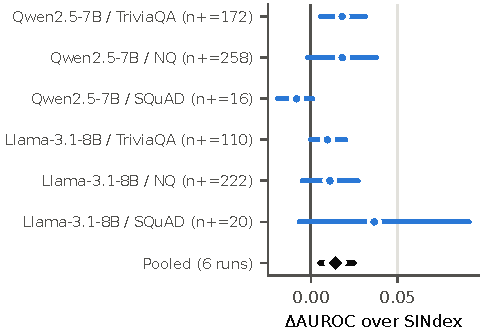
\includegraphics[width=\columnwidth]{figures/forest.pdf}
\caption{Per-run AUROC gain of the NLI veto over SINdex with 95\% bootstrap intervals, and the pooled estimate. $n_+$: number of hallucinated answers under validated labels.}
\label{fig:forest}
\end{figure}

\begin{figure}[t]\centering
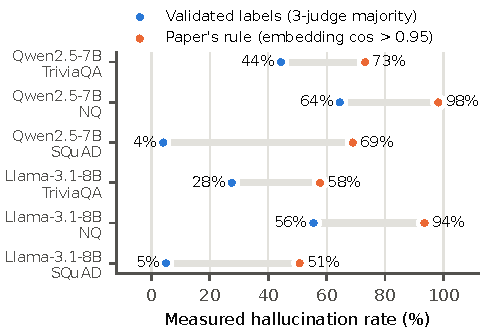
\includegraphics[width=\columnwidth]{figures/label_rates.pdf}
\caption{Measured hallucination rate under the paper's labelling rule vs.\ validated labels. The embedding rule marks many correct but verbose answers as hallucinations.}
\label{fig:labelrates}
\end{figure}

\textbf{Contradiction-aware clustering helps.} With validated labels (Table~\ref{tab:main}, Fig.~\ref{fig:forest}), adding the NLI veto gives the best black-box AUROC in 5 of 6 settings and is significantly better than SINdex on Qwen/TriviaQA, Qwen/NQ and Llama/TriviaQA. Pooled over all six runs (Table~\ref{tab:pooled}) the gain is $+0.014$ AUROC (95\% CI $[+0.005,+0.025]$, $p<0.001$); with consensus labels it is $+0.017$ ($[+0.004,+0.032]$, $p=0.002$). The single setting without a gain, Qwen/SQuAD, has only 4\% hallucinations (16 of 400), so its AUROC is estimated from very few positives.

\textbf{SINdex's advantage depends on its labels.} Table~\ref{tab:labeleffect} and Fig.~\ref{fig:labelrates} show that the embedding rule inflates the measured hallucination rate by a factor of 1.5--2.1 on TriviaQA and NQ and by a factor of 10 or more on SQuAD, where the model reads the passage and is almost always right. Under the paper's labels SINdex leads plain cluster entropy by $+0.040$ AUROC pooled ($p<0.001$); under validated labels the lead is $+0.007$ and not significant ($p=0.21$). SINdex is also statistically tied with the EigV baseline of~\cite{lin2024generating} ($+0.006$, $p=0.08$). The effect is larger for Qwen, whose answers are longer full sentences, than for Llama, which answers more tersely; the embedding rule penalises verbosity.

\textbf{SINdex++ corrects the theory but not the ranking.} On Qwen/TriviaQA, SINdex++ differs from SINdex on 255 of 388 questions, and SINdex falls below $H(p)$ on 59 of them, the violation of Proposition~\ref{prop:flaw} in practice. Yet the pooled AUROC difference is $+0.000$ ($[-0.001,+0.001]$). At a cut of cosine $0.95$, cohesion inside non-singleton clusters is close to 1, so both cohesion terms are small relative to $H(p)$. We therefore recommend SINdex++ for its guarantees and well-defined singleton handling, not for accuracy.

\textbf{Negative results.} The adaptive cut reduces the number of clusters (e.g., from 3.3 to 1.7 per question on Qwen/TriviaQA) but merges answers that should stay apart, lowering AUROC by $0.020$ pooled. Early stopping saves 16--65\% of the samples (3.5--8.4 of 10 used on average) but costs $0.020$ AUROC pooled. Both use untuned settings; tuning them on a separate validation split is left to future work.

% =====================================================================
\section{Discussion and Limitations}
\textbf{Implications for evaluation.} Automatic labels that compare a free-form answer with a short reference by embedding similarity or exact match systematically mislabel correct, verbose answers. Because verbosity varies across models and prompts, such labels can create or remove differences between detectors. We recommend validating labelling rules against a manually checked sample before reporting detector comparisons, and releasing the labels.

\textbf{Limitations.} (1)~The reference annotation was produced with LLM assistance; it was confirmed by one human on a 40-item random subset, and a second independent annotator would strengthen it. (2)~We evaluate two 7--8B open models and 400 questions per dataset; larger models and full test sets may behave differently. (3)~We did not re-implement NLI-based semantic entropy~\cite{farquhar2024detecting} or kernel language entropy~\cite{nikitin2024kernel}; our conclusions concern SINdex relative to embedding-based baselines. (4)~The judges include a model from the same family as one generator; the cross-family judge (Granite) agrees with the reference most closely, which mitigates but does not exclude self-preference. (5)~SQuAD with context yields too few hallucinations for reliable AUROC with these models. (6)~We report results only for short-answer QA.

% =====================================================================
\section{Conclusion}
SINdex's cohesion-weighted entropy is not monotone in cohesion as claimed; SINdex++ fixes this with provable guarantees but no change in accuracy. The embedding-cosine labels used to evaluate SINdex are close to chance against a validated reference, and under validated labels SINdex performs on par with plain cluster entropy and with an earlier graph-based baseline. A targeted fix to the clustering, vetoing merges of borderline-similar answers that an NLI model finds contradictory, gives a small but consistent improvement across two models and three datasets. We release code, generations, labels and annotations to support validated evaluation of hallucination detectors.

\section*{Data and Code Availability}
Code, all sampled generations, scores, labels (including each judge's raw output) and the reference annotations are available at \todo{public repository URL}.

\section*{Acknowledgment}
\todo{Funding / institutional acknowledgment.} The authors used Claude (Anthropic) to assist with software development, the reference annotation described in Section~\ref{sec:labels} (verified by a human annotator), and drafting of this manuscript; the authors reviewed and take responsibility for all content. \todo{Confirm this disclosure matches IEEE's policy on AI-generated content and your actual use.}

\bibliographystyle{IEEEtran}
\bibliography{refs}

\end{document}
